\documentclass[10pt,twocolumn,letterpaper]{article}

\usepackage{cvpr}
\usepackage{times}
\usepackage{epsfig}
\usepackage{graphicx}
\usepackage{amsmath}
\usepackage{amssymb}
\usepackage[lined,algonl,boxed]{algorithm2e}
\usepackage{algorithmic}

% Include other packages here, before hyperref.

% If you comment hyperref and then uncomment it, you should delete
% egpaper.aux before re-running latex.  (Or just hit 'q' on the first latex
% run, let it finish, and you should be clear).
\usepackage[pagebackref=false,breaklinks=true,letterpaper=true,colorlinks,bookmarks=false]{hyperref}

\newcommand{\todd}[1]{\textcolor{red}{[\bf TZ: #1]}}
\newcommand{\ruonan}[1]{\textcolor{blue}{[\bf RL: #1]}}

%\cvprfinalcopy % *** Uncomment this line for the final submission

\def\cvprPaperID{1332} % *** Enter the CVPR Paper ID here
\def\httilde{\mbox{\tt\raisebox{-.5ex}{\symbol{126}}}}

% Pages are numbered in submission mode, and unnumbered in camera-ready
\ifcvprfinal\pagestyle{empty}\fi

\begin{document}

%%%%%%%%% TITLE
\title{Supplemental Material Accompanying Paper 1332,\\ ``Finding Group Interactions in Social Clutter''}
%\author{ Ruonan Li and Todd Zickler\\
%Harvard School of Engineering and Applied Science\\
%{\tt\small \{ruonanli,zickler\}@seas.harvard.edu}
%}

\maketitle
% \thispagestyle{empty}


\section{Details of Branch-and-Bound Localization}
\label{detailBB}

To apply branch-and-bound algorithm to minimize (\ref{quality}), we first specify the spaces where $T_{s}$ and $T_{e}$ may take a value. We denote the length of the shortest exemplar activity as $T_{min}$, then we assume $1\leq T_{s}\leq T-T_{min}+1$ and $T_{min}+1\leq T_{e}\leq T$. Additional constraint may be imposed, such as $T_{min}\leq T_{e}-T_{s}$. Given these information,  the temporal branch-and-bound algorithm, as a companion to the 2-D case studied in \cite{Lampert}, can be derived as in Algorithm \ref{Algo:2}.  In this algorithm, $\hat{f}(T_{s,low}, T_{s,upp}, T_{e,low}, T_{e,upp})$ is a lower bound of the values of the quality function evaluated on all intervals enclosed in $[T_{s,low}, T_{s,upp}]\times [T_{e,low}, T_{e,upp}]$. To calculate this lower bound, we define
\begin{equation}
\begin{split}
&\hat{f}(T_{s,low}, T_{s,upp}, T_{e,low}, T_{e,upp})\\
&=\sum^{L-1}_{l=0}\sum^{2^{l}}_{i=1} \hat{f}(T^{l,i}_{s,low}, T^{l,i}_{s,upp}, T^{l,i}_{e,low}, T^{l,i}_{e,upp})
\end{split}
\end{equation}
where $T^{i,l}_{s}, T^{i,l}_{e}$ are the boundaries of cell $\mathcal{C}(T_{s},T_{e}, l,i)$. In other words, we use the summation of the lower bounds of all cells in the pyramid as the lower bound of the entire interval. The evaluation of $\hat{f}(T^{l,i}_{s,low}, T^{l,i}_{s,upp}, T^{l,i}_{e,low}, T^{l,i}_{e,upp})$, however, is a $\mathcal{O}(1)$ operation with the help of integral dissimilarities $I(t)$ of those negative group dissimilarities $D^{*}(t)$ over $t$. Specifically, let
\begin{equation}
I(t)=\sum^{t}_{t'=1} \min(0,D^{*}(t))
\end{equation}
which only needs to be computed once. Then the lower bound for the cell $\mathcal{C}(T_{s},T_{e}, l,i)$ can be obtained as
\begin{equation}
\hat{f}(T^{l,i}_{s,low}, T^{l,i}_{s,upp}, T^{l,i}_{e,low}, T^{l,i}_{e,upp})=I(T^{l,i}_{e,upp})-I(T^{l,i}_{s,low}).
\end{equation}


\begin{algorithm*}[h]
\begin{enumerate}
\footnotesize{
\item Initialize: Let $T_{s,low}=1$, $T_{s,upp}=T-T_{min}+1$, $T_{e,low}=T_{min}+1$, and $T_{e,upp}=T$; Initialize priority queue $Q$ as empty; 
\item Do
\begin{itemize}
\item If $T_{s,upp}-T_{s,low} \ge T_{e,upp}-T_{e,low}$\\
$T^{(1)}_{s,low}\leftarrow T_{s,low}$, $T^{(1)}_{s,upp}\leftarrow T_{s,low}+\frac{T_{s,upp}-T_{s,low}}{2}$,
$ T^{(1)}_{e,low}\leftarrow T_{e,low}$, $T^{(1)}_{e,upp}\leftarrow T_{e,upp}$,
$T^{(2)}_{s,low}\leftarrow T_{s,low}+\frac{T_{s,upp}-T_{s,low}}{2}$, $T^{(2)}_{s,upp}\leftarrow T_{s,upp}$,
$ T^{(2)}_{e,low}\leftarrow T_{e,low}$, $T^{(2)}_{e,upp}\leftarrow T_{e,upp}$;\\
else \\
$T^{(1)}_{s,low}\leftarrow T_{s,low}$, $T^{(1)}_{s,upp}\leftarrow T_{s,upp}$,
$ T^{(1)}_{e,low}\leftarrow T_{e,low}$, $T^{(1)}_{e,upp}\leftarrow T_{e,low}+\frac{T_{e,upp}-T_{e,low}}{2}$,
$T^{(2)}_{s,low}\leftarrow T_{s,low}$, $T^{(2)}_{s,upp}\leftarrow T_{s,upp}$,
$ T^{(2)}_{e,low}\leftarrow T_{e,low}+\frac{T_{e,upp}-T_{e,low}}{2}$, $T^{(2)}_{e,upp}\leftarrow T_{e,upp}$;
\item If $T_{min}\leq T^{(1)}_{e,upp}-T^{(1)}_{s,low}$,
push $(T^{(1)}_{s,low}, T^{(1)}_{s,upp}, T^{(1)}_{e,low}, T^{(1)}_{e,upp},\hat{f}(T^{(1)}_{s,low}, T^{(1)}_{s,upp}, T^{(1)}_{e,low}, T^{(1)}_{e,upp}))$ into $Q$;\\
\item If $T_{min}\leq T^{(2)}_{e,upp}-T^{(2)}_{s,low}$,
push $(T^{(2)}_{s,low}, T^{(2)}_{s,upp}, T^{(2)}_{e,low}, T^{(2)}_{e,upp},\hat{f}(T^{(2)}_{s,low}, T^{(2)}_{s,upp}, T^{(2)}_{e,low}, T^{(2)}_{e,upp}))$ into $Q$;\\
\item Let $(T_{s,low}, T_{s,upp}, T_{e,low}, T_{e,upp})$ be the tuple in $Q$ achieving the minimal $\hat{f}$;
\end{itemize}
Until $T_{s,low}=T_{s,upp}, T_{e,low}=T_{e,upp}$.
\item Output: $T_{s}\leftarrow T_{s,low}, T_{e}\leftarrow T_{e,low}$. 
}
\end{enumerate}
\caption{\small Branch-and-bound search for temporal localization.}
\label{Algo:2}
\end{algorithm*}

\section{Details for Classroom Interaction Dataset}

The raw video framerate is 15fps.

We have applied an OpenCV face detector and generated long tracks of the bounding boxes using a combination of OpenCV mean-shift tracking and dominant optical flows. We manually eliminate the false-alarm boxes/tracks and recover (very few) miss-detections when using the video for building ground-truth exemplars, and do not involve manual correction when testing our approach. 


In consultation with education experts we define interaction categories based on the geometric configurations of the participants: three categories for 2-person interactions (same row; different rows with left agent in front; different rows with right agent in front) and four categories for 3-person interactions (three people in the same row with two looking left; three people in the same row with two looking right; two people in back row with one in front; two people in front row with one behind). Examples of these images are shown in Fig.~\ref{dataset}.
\begin{figure}[h]
\begin{center}
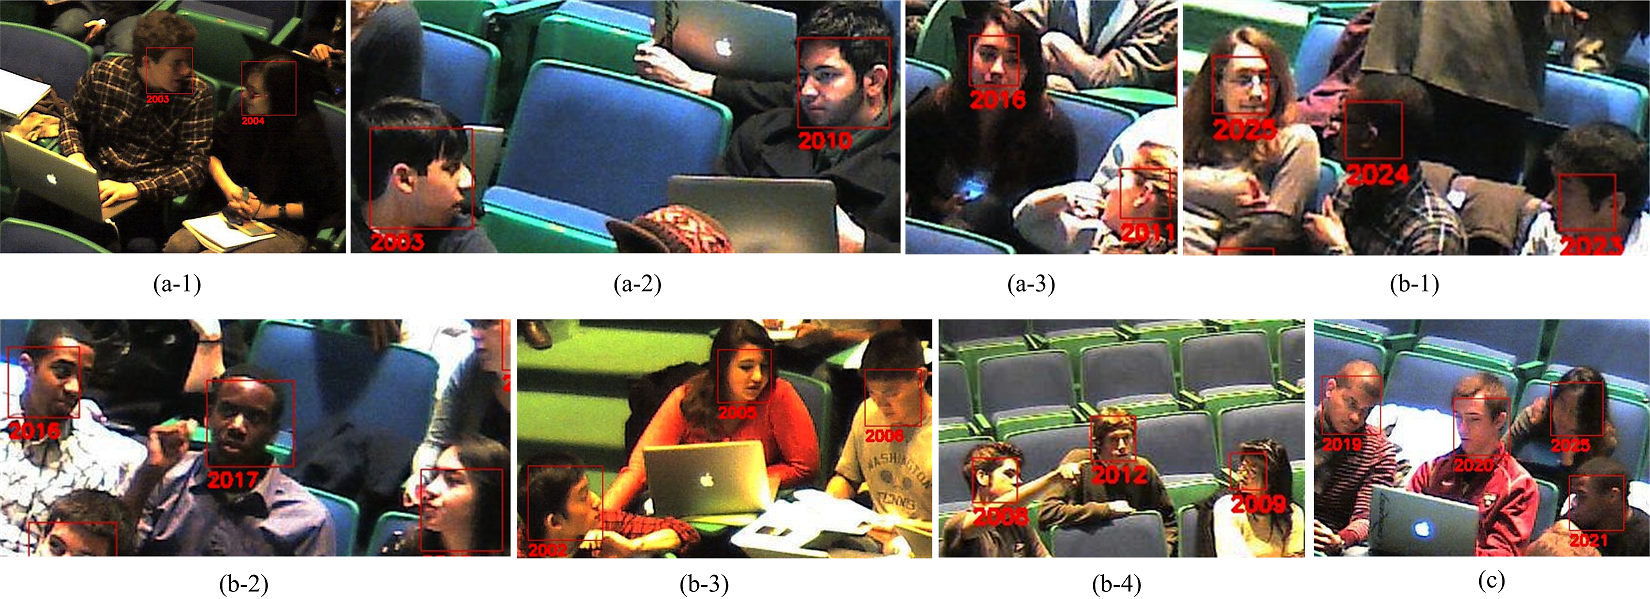
\includegraphics[scale=1.2]{dataset.png}
\end{center}
\caption{Samples of two-person ((a-1)(a-2)(a-3)), three-person ((b-1)(b-2)(b-3)(b-4)), and four-person (c) interactions in the classroom interaction dataset we collected.}
\label{dataset}
\end{figure}


\subsection{Descriptors}

We use a coarse representation of the head pose as the individual descriptor. Specifically, we compute the Histogram of Oriented Gradient (HOG) feature within each temporal unit and each box, and apply nine one-against-all SVMs to estimate the likelihood of a HOG feature belonging to nine head poses (front, left, lower-left, lower-front, lower-right, right, back-right, and back-left). The nine-dimensional likelihood vector  serves as our individual descriptor. Meanwhile, we derive the pairwise descriptor for three or more individuals based on the geometrical configurations of the bounding boxes. As shown in the left panel of Figure \ref{all_illu}(b), where a descriptor of target $m$ relative to target $m'$ among five targets at time $t$ is computed, we compute the distances $r_{i}$'s between all others and $m$, and the relative angles $a_{i}$'s between the connecting vectors and $\overrightarrow{mm'}$, and combine all these geometric quantities into a pairwise descriptor $\mathbf{g}_{m,m',t}$. When computing $\mathbf{g}_{n,n',s}$ in the input (right panel of Figure \ref{all_illu}(b)), we align $\overrightarrow{nn'}$ against $\overrightarrow{mm'}$ and predict the locations of the three individuals (shown in red), and compute the true distances $z_{i}$'s and relative angles $b_{i}$'s by locating the nearest individuals to the predicted locations. This pairwise representation achieves invariance under similarity transforms. For two-person interaction, we simply use the distance and the relative angles against the right horizontal axis (Figure \ref{all_illu}(c)). 

\begin{figure}[t]
\begin{center}
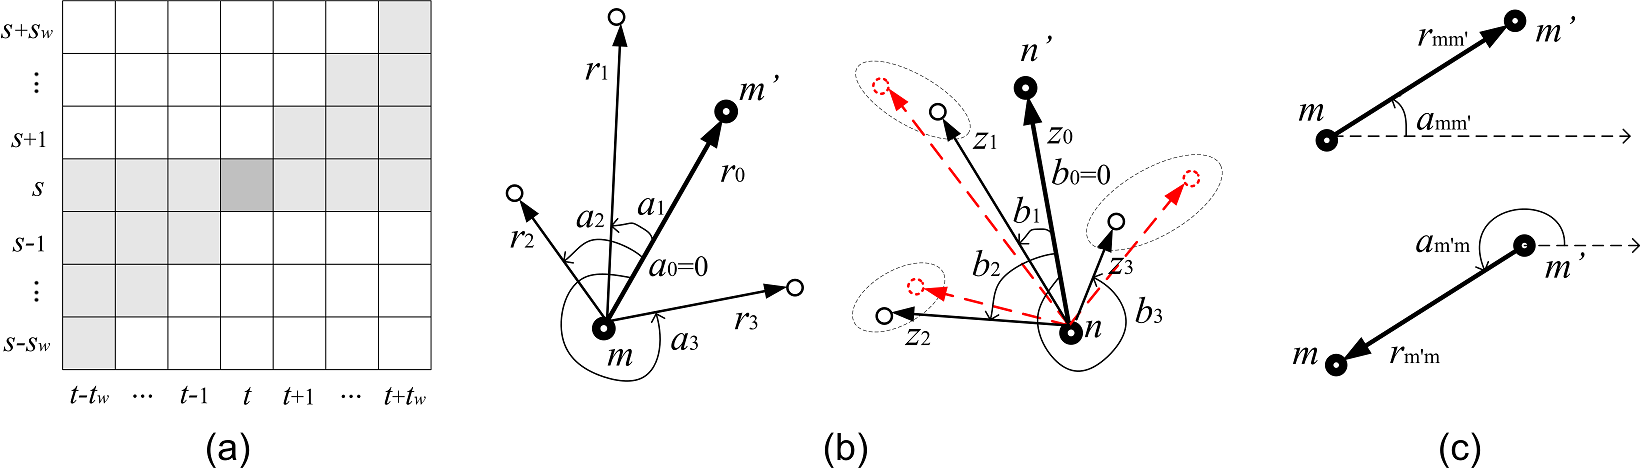
\includegraphics[scale=1.2]{all_illu.png}
\end{center}
\caption{For the classroom dataset, pairwise descriptors for groups comprised of (a) three or more participants, and (b) two participants. See text for details. \todd{Remove the left part of this figure}}
\label{fig:classroom-pairwise}
\end{figure}

\subsection{Computational cost}

We first look into the computational cost. We replace the optimal matching method with an exhaustive enumeration of all possible matchings. We also apply temporal sliding windows at eight scales ranging from half to twice of the exemplar length, stopping using the remaining scales whenever the current window achieves the same quality function value as the branch-and-bound. We show the average computation time for one match between an exemplar and an input on a 8-core 2.8GHz Macintosh in Table \ref{computecost} (supplementary material), where we see clear savings for the proposed approach.


\begin{table}[h]
\centering \caption{Computational cost comparison for the proposed matching approach and baselines (in seconds).}
\footnotesize{
\begin{tabular}{|c|c|c|c|}
\hline    \# of Participants &  2  &  3  &  4   \\
\hline   Exhaustive+Sliding Window & 17.2   & 60.4   & 253.2   \\
\hline  Exhaustive+Branch and Bound &  12.6 &  27.6  &   59.7 \\
\hline  Optimal Pairing+Sliding Window & 12.4  & 23.2   &  40.8  \\
\hline  Proposed & 8.0  &  19.8  &  32.3  \\
\hline 
\end{tabular}
}
\label{computecost}
\end{table}

\subsection{Temporal localization}
We finally investigate the temporal localization performance, for which we compute the ratio of the intersection to the union of the estimated interval and the annotated interval, and show the averages in Figure \ref{classtemporal}(b).  Again, metric learning improves the capability of finding temporal boundaries.

\begin{figure*}[t]
\begin{center}
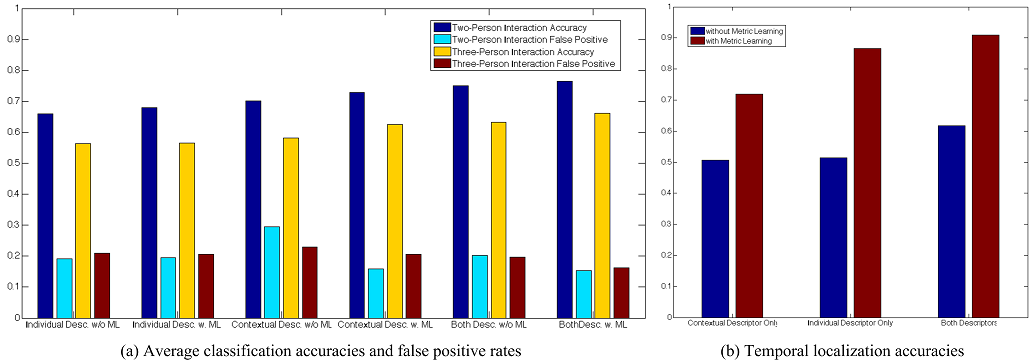
\includegraphics[scale=2.5]{classtemporal.png}
\end{center}
\caption{Average classification accuracies and false positives for two-person and three-person interactions (Individual and/or pairwise descriptors, with or without metric learning (ML)) and the temporal localization accuracies.}
\label{classtemporal}
\end{figure*}

\subsection{More examples}

\todd{If you reduce the number of results included in the main paper, you could include some more here.}

\begin{figure*}
\begin{center}
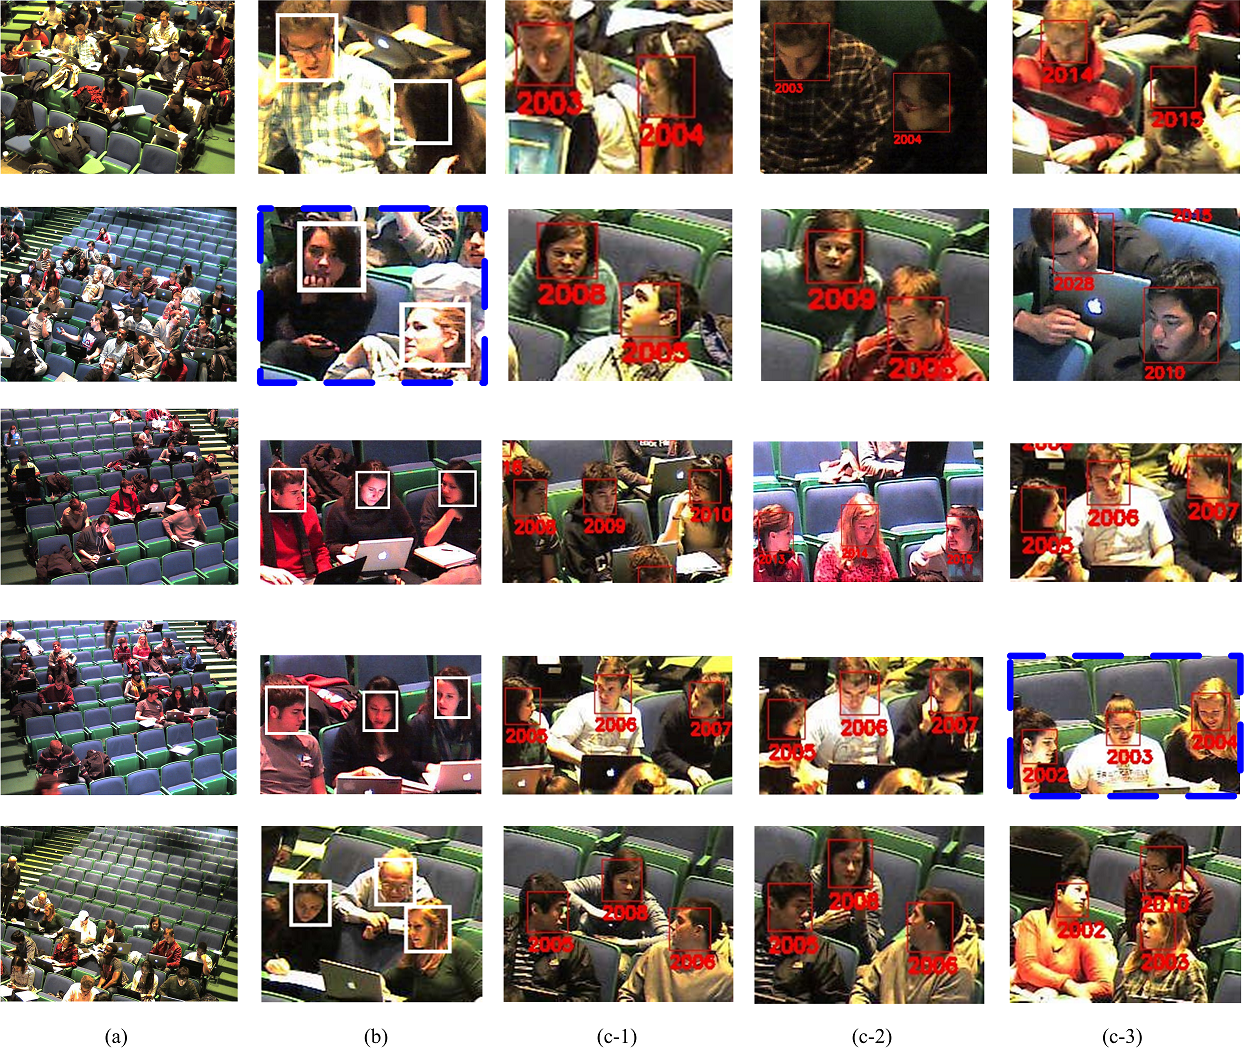
\includegraphics[scale=2.25]{retrieved.png}
\end{center}
\vspace{-10pt}
\caption{Examples of social interaction detection and matching on the classroom interaction database. Each row is an example of detecting a salient interaction from an input and enumerating similar database exemplars: (a) is the input, (b) is the detected social interaction, and (c-1) to (c-3) are the top three associated database exemplars that support this detection.}
\label{retrieved}
\end{figure*}

\subsubsection{UT-Interaction Dataset}


\begin{table}[h]
\centering \caption{Classification accuracies and false positive (FP) rates comparison on UT-Interaction dataset for evaluating the effectiveness of different components of the proposed approach: Individual and/or pairwise descriptors, with or without metric learning (ML).}
\footnotesize{
\begin{tabular}{|c|c|c|c|}
\hline   & Individual only & pairwise only & Both \\
\hline Accur. w. ML & 0.688 & 0.813 & 0.854  \\
\hline Accur. w/o ML & 0.647 & 0.750 & 0.771    \\
\hline FP Rate w. ML &  0.125 & 0.096 & 0.071  \\
\hline FP Rate w/o ML & 0.163 & 0.113 & 0.083\\
\hline 
\end{tabular}
}
\label{UTaccuFPdegrade}
\end{table}


\subsubsection{Caltech Resident-Intruder Mouse Dataset.} 

We also tested the approach on Caltech Resident-Intruder Mouse Dataset \cite{CRIM13}, which contains long video sequences recording pair-wise interactions between two mice. Behaviors are categorized into 12 different mutually exclusive action types, plus an `other' category indicating no behavior of interest is occurring. A video typically lasts around 10 minutes at 25fps with a resolution of 640x480 pixels. Every video frame is labeled with one of the thirteen ground-truth categories, resulting in a segmentation of the videos
into action intervals. For more details please refer to \cite{CRIM13}. Note that in all videos are pair-wise interactions, and our experiment on this dataset is not meant to distinguish the participants, but to demonstrate that our approach can be directly used for a traditional task of temporal segmentation and classification without any changes.

We exactly follow the training/testing partitions provided by the dataset. We extract the spatio-temporal interest points (STIP) based appearance features and compute trajectory-based features from the tracks provided with the dataset as \cite{CRIM13} does (See \cite{CRIM13} for details). Differently from \cite{CRIM13}, we only compute STIP based features inside the bounding boxes enclosing the mice. The trajectory-based features consists of those describing the motion of each individual mouse and those describing the relative motion between two mice. We denote the former as T\_ind and the latter as T\_pair. Again we use a 4-level temporal pyramid, in which the STIP based appearance features are computed as \cite{CRIM13} does and the trajectory based features are also transformed into histograms against 64 codewords. 

Three combinations of features were attempted in \cite{CRIM13}: Trajectory only, STIP only, and using both. For the case trajectory only, our approach has two possible working modes: Using all trajectory-based features as individual descriptors (denoted as Trajectory\_1), or using T\_ind as individual descriptors and using T\_pair as pairwise descriptors (denoted as Trajectory\_2). In the case of STIP only, all features are used as individual descriptors, and in the case of using both, STIP features and trajectory-based features serve as individual descriptor and pairwise descriptors respectively. To classify a segment responded by one or more exemplars, we simply give it the label of the top-ranked exemplar. We follow the same error metric as \cite{CRIM13}, the frame-wise accuracy, and report the results in Table \ref{CRIMAccu}, where it is evident that motion trajectory is much more discriminative than local STIP based features given little articulation in a constrained environment. The competing performance by approach is achieved by splitting the motion into individual ones and pairwise ones and learning separate metrics for them (Trajectory\_2). In other cases, multi-level adaboost based approach exhibits superiority on frame-wise classifications (as in \cite{CRIM13}).


\begin{table}[h]
\centering \caption{Accuracies for the proposed method and the baselines on Caltech Resident-Intruder Mouse Dataset. (\%)}
\footnotesize{
\begin{tabular}{|c||c|c|c|c|}
\hline   & Trajectory\_1  & Trajectory\_2 & STIP & Both \\
\hline \cite{CRIM13} w/o. context & 52.3  & 52.3 & 29.3 & 53.1\\
\hline \cite{CRIM13} w. context &  \underline{58.3} & 58.3 & \underline{43.0} & 61.2\\
\hline Ours w/o. ML &  45.6 & 49.4 & 18.8 & 50.9 \\
\hline Ours w. ML & 54.5 & \underline{66.0} & 31.7 & \underline{62.9}\\
\hline 
\end{tabular}
}
\label{CRIMAccu}
\end{table}

It is observed in \cite{CRIM13} that accuracy varies with the length of the interaction and with the length of window within which the local feature is computed. To investigate the performance of our approach on different lengths of the interaction as compared to \cite{CRIM13}, we implemented the approach in \cite{CRIM13} using trajectory-based features and one-level auto-context classifier. As shown by the result in Figure \ref{frame_no}, our approach is particularly better at localizing longer interactions though \cite{CRIM13} demonstrates its advantage under a shorter feature window on shorter interactions. 

\begin{figure}[h]
\begin{center}
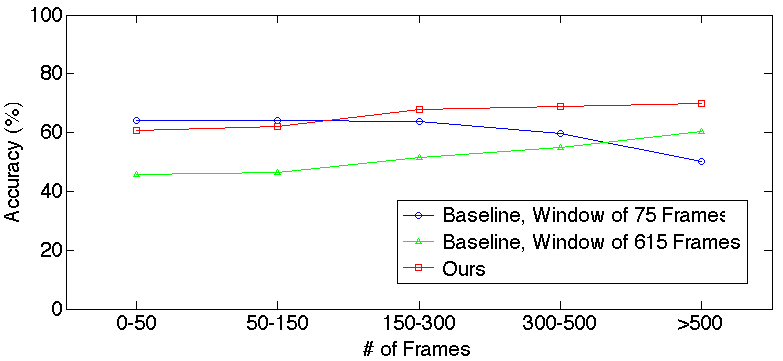
\includegraphics[scale=0.25]{frame_no.png}
\end{center}
\caption{Accuracy comparison for varying length of interactions between \cite{CRIM13} and our approach.}
\label{frame_no}
\end{figure}


\bibliographystyle{ieee}
{\footnotesize
\bibliography{egbib}
}

\end{document}
